
 \section{Beschrijving}
 De resultaten van het onderzoek, dat hierboven beschreven wordt, bestaan vooral uit grafieken, waaruit een juiste waarde voor \textit{C\tss{g}} wordt afgelezen. Die grafiek wordt verkregen door de formule (blz 109 uit het boek van Rabae [1])
 \begin{equation}
 I = C_g(V\tss{GS}) \frac{dV\tss{GS}}{dt}
 \end{equation}
 om te schrijven naar:
 \begin{equation}
 C_g(V\tss{GS})= \frac{I}{ \frac{dV\tss{GS}}{dt}}
 \end{equation}
 Deze functie kun je uit laten rekenen door SPICE. Dan komt er de volgende grafiek uit: (figuur \ref{res:1}) 
 \begin{figure} [h!]
 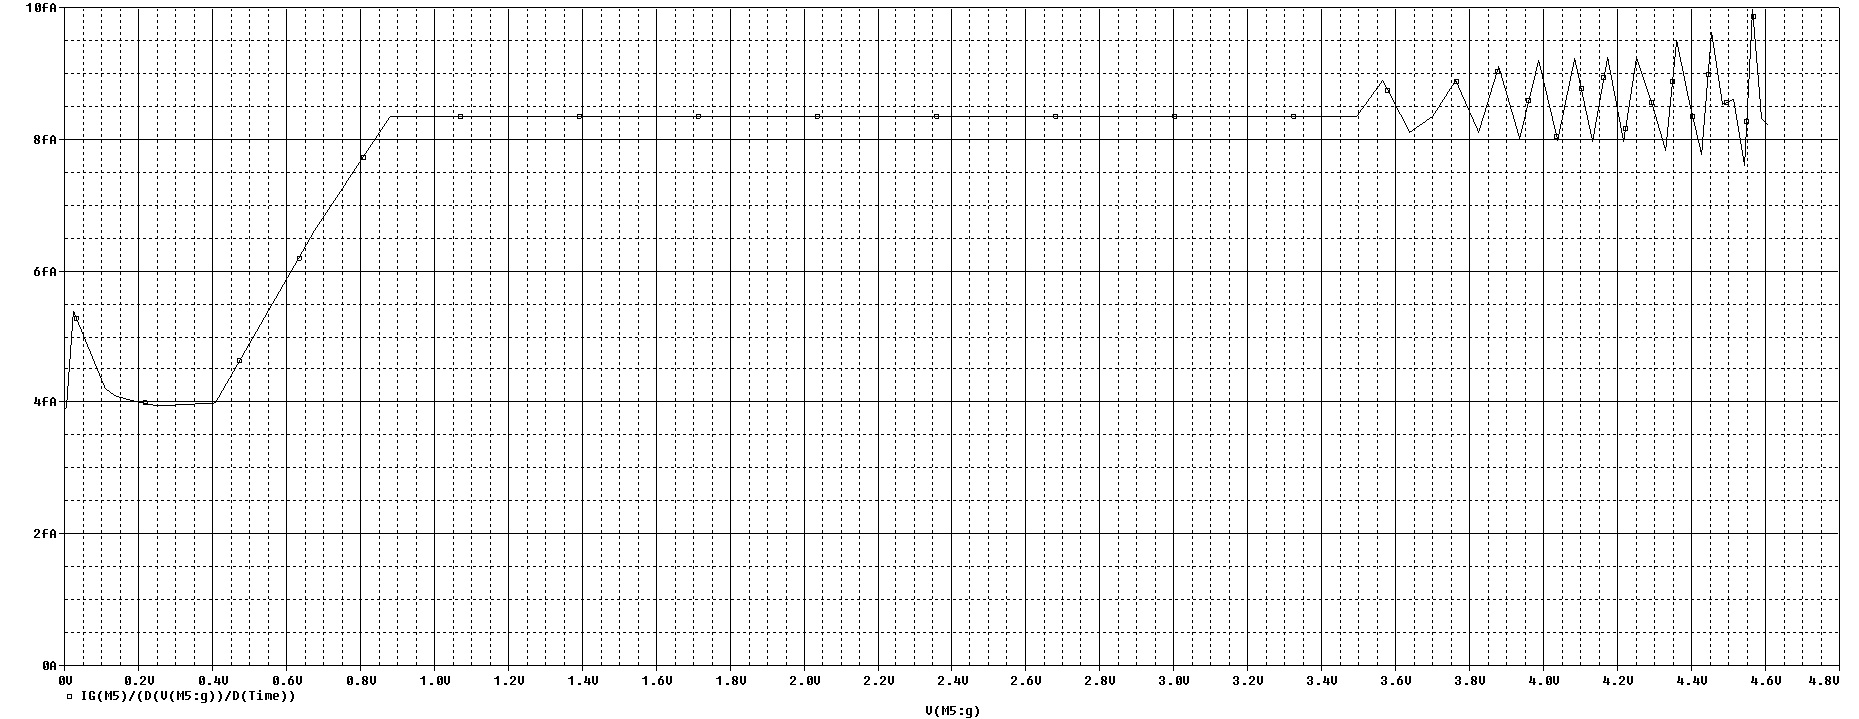
\includegraphics [width = \textwidth] {Graphs_nmos/C_L_2_2}
 \caption{$C_g$ als functie van V\tss{GS} met W=3um en L = 2.2um.}
 \label{res:1}
 \end{figure}
 Vervolgens kun je SPICE de capaciteit laten bepalen. Dit is het vlakke deel van de grafiek in figuur \ref{res:1}. Zowel voor  de NMOS als voor de PMOS is dit gedaan voor verschillende waarden van L. De strategie is hierboven al beschreven, maar de formule voor de totale gate capaciteit verduidelijkt veel. Deze komt uit de projectopdracht. 
 \begin{equation} \label{res:eq1}
 C_g = W *C_0 + L *W *C\tss{GC}
 \end{equation}
 Wanneer W vastgezet wordt en L gevarieerd wordt, verkrijgt men een lineair verband. Voor dezelfde waardes van W en bij verschillende waardes van L is steeds de totale capaciteit bepaald. De resulaten voor zowel de NMOS als de PMOS transistor staan in figuur \ref{res:2}.
 \begin{figure} [h!]
 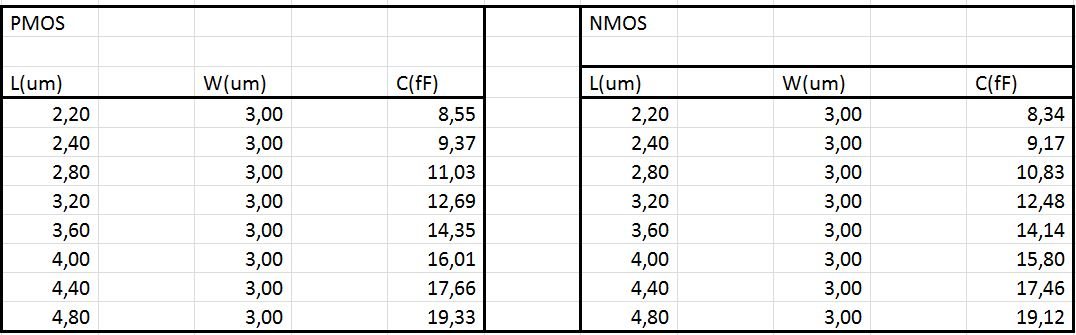
\includegraphics [scale = 0.4] {figures/tabel}
 \caption{De door SPICE berekende waarden van $C_g$ bij veranderende L}
 \label{res:2}
 \end{figure}
 Zoals eerder gezegd, wordt een lineair verband tussen \textit{$C_g$}en L verwacht. Wanneer we deze plotten in Matlab (appendix  \ref{M1}) zien we inderdaad een lineair verband, zowel voor de NMOS als voor de PMOS. Met de "Basic Fitting" functie van Matlab werden beide functies bepaald. Die staan onder de figuren \ref{res:3} en \ref{res:4}.
 
 \begin{figure} [h!]
 \centering
 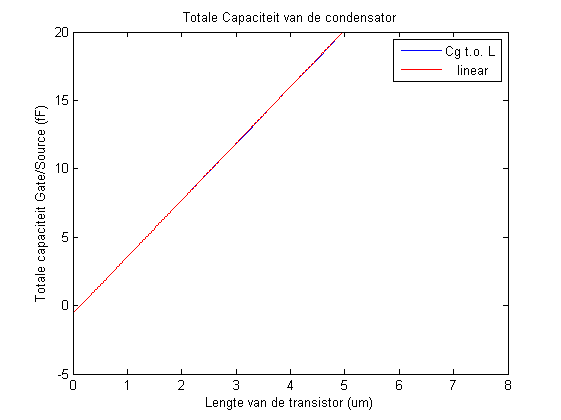
\includegraphics [scale = 0.4] {figures/c0.png}
 \caption{$C_g$ vs L, 4.1449x  - 0.78078 voor de NMOS}
 \label{res:3}
 \end{figure}
 
 \begin{figure} [h!]
 \centering
 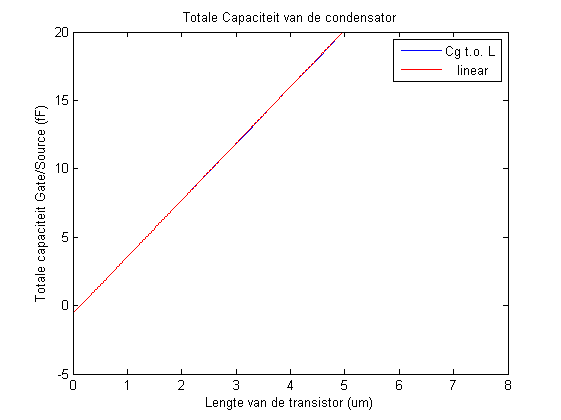
\includegraphics [scale = 0.4] {figures/c0p.png}
 \caption{$C_g$ vs L, 4.1464x  - 0.57784 voor de PMOS}
 \label{res:4}
 \end{figure}
 Het uiteindelijke doel is om \textit{C\tss{GC}} te bepalen in vergelijking \ref{res:eq1}. Je kunt \textit{C\tss{0}*W} aflezen uit de grafiek.(in figuur \ref{res:3} en \ref{res:4})  \textit{C\tss{0 }*W} is dan de plaats waar de lijn de y-as snijdt. Die zijn voor de NMOS en de PMOS respectievelijk -0.7808 en -0.5778. (zie figuur \ref{res:3} en \ref{res:4}) \textit{C\tss{GC}} is te bepalen door vergelijking \ref{res:eq1} om te schrijven. Dat staat in \ref{res:eq2}:
 \begin{equation} \label{res:eq2}
C\tss{GC} = \frac{C_g - C_0*W}{W*L}
 \end{equation}
 
Dan kan \textit{C\tss{GC}} dus bepaald worden. (bij een gekozen L) Hierbij moet vermeld worden dat \textit{C\tss{GC}} de capaciteit per oppervlakte is. In vergelijking \ref{res:eq3} staat de mogelijkheid om de dikte van het gateoxide te berekenen. Dit is de algemene formule voor een vlakke plaatcondensator. \textit{$\epsilon$\tss{ox}} is de waarde die in het boek [1] gegeven is. 
 \begin{equation} \label{res:eq3}
 C\tss{GC}*A = \frac { \epsilon\tss{ox} A } {d}
 \end{equation}
 Vervolgens kun je de A wegstrepen, waaruit de dikte dan te berekenen is. Om C\tss{GC} en deze dikte snel te kunnen berekenen, is even een matlabcode geschreven. (appendix \ref{M2}). De diktes van de gateoxides van de PMOS en de NMOS voor random waardes van L tussen 2.2 en 4.8 staan in tabel \ref{res:tab1}.
 \begin{table} [h!]
  \begin{tabular}{ | c |c| } 
 \hline
   Dikte gateoxide PMOS (nm) & Dikte gateoxide NMOS (nm) \\ \hline
     24.759 &  25.329  \\ \hline
      24.983 &    25.335 \\ \hline
       25.062 &   25.327\\ \hline
     
 \end{tabular}
 \caption{Diktes van gateoxide van de gesimuleerde NMOS en PMOS transistors}
 \label{res:tab1}
  \end{table}
 \section{Analyse}
 \subsection{Bespreking grafiek in figuur \ref{res:1} }
 In deze figuur wordt C als functie van V\tss{GS} geplot. Daarbij is er eerst een dal te zien, waarna de \textit{$C_g$} eerst  naar een stabiele waarde gaat en later gaat oscilleren.   Het dal wordt verklaard door de situatie dat de gate-source spanning eerst klein is en naarmate \textit{V\tss{GS}} groter wordt steeds meer positieve ladingsdragers (ofwel gaten) wegduwt, waardoor het depletiegebied groter wordt. Hierdoor wordt de capaciteit kleiner, volgens de algemene formule voor de capaciteit van een plaatcondensator (eq.\ref{res:eq3}). Hiermee kun je de dip verklaren. Vervolgens wordt \textit{V\tss{GS}} zo groot, dat ze boven de drempelspanning uitkomt. Dan ontstaat er een inversiegebied, waarin geleiding mogelijk is. Dan is het depletiegebied weer kleiner, waardoor de capaciteit omhoog gaat naar een constante waarde en de grafiek een constante lijn vertoont. Als \textit{V\tss{GS}} echt groot wordt, treedt er een soort oscilatie op, te verklaren door snelheidsverzadigingseffecten. Bij elke van de gekozen waarden van L tussen 2.2 en 4.8 $\mu$m ontstond er een soortgelijke grafiek. 
 \subsection{Bespreking uitkomsten}
 In dit onderdeel wordt bekeken of er realistische waarden uit  de berekeningen komen. De diktes van de gateoxides van de NMOS en de PMOS zijn  vooral in termen van nanometer. Dat klopt, in moderne processen is men van 300nm (dikte) voor 10$\mu$m (L) technologie naar 1.2nm voor 65nm technologie gegaan.[2] Onze NMOS en PMOS zijn voor deze tijd (2013, in de orde van $\mu$m, in plaats van nm) erg groot en zullen dus meer nanometer zijn. In figuur \ref{res:5} staat nog een plaatje van de diktes van het gateoxide als functie van L. 
\begin{figure} [h!]
  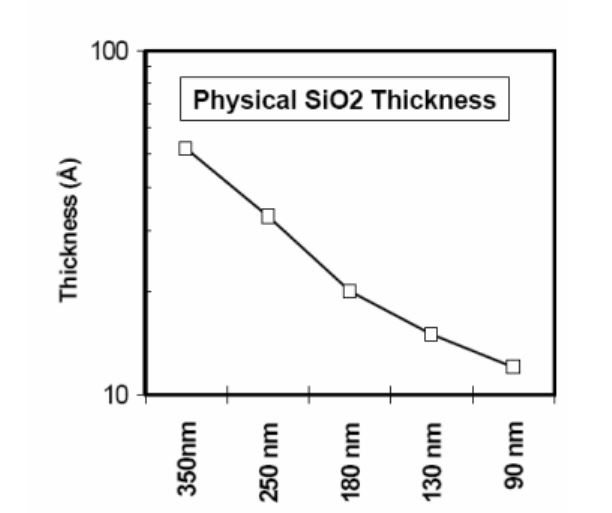
\includegraphics [scale = 0.3] {figures/sio2.jpg}
 \caption{Dikte gateoxide, uitgezet tegen de lengte van de NMOS [2]}
 \label{res:5}
\end{figure}
\newpage
Uit de berekeningen van \textit{C\tss{GC}} komen vooral waardes in  de ordegrootte femtofarad. Dat is een realistische capaciteit voor zowel de NMOS als de PMOS transistor. [3] Uit dit artikel blijkt ook dat er nog veel meer capaciteiten zijn dan alleen \textit{C\tss{GC}} , maar daar gaat het bij discussie nog over. \\
Verder zou je je nog af kunnen vragen of de dikte van het gate oxide afhankelijk is van de lengte van de transistor. Aan figuur \ref{res:tab1} is te zien dat de dikte onafhankelijk is van L. Dit komt omdat vergelijking \ref{res:eq2} een lineaire functie is. 

 

